\begin{figure*}[t]
	\centering
	\begin{tabular}{cccc}
		\hspace{-0.55em}\subfloat[][$\Delta=1\times10^{-2}$]{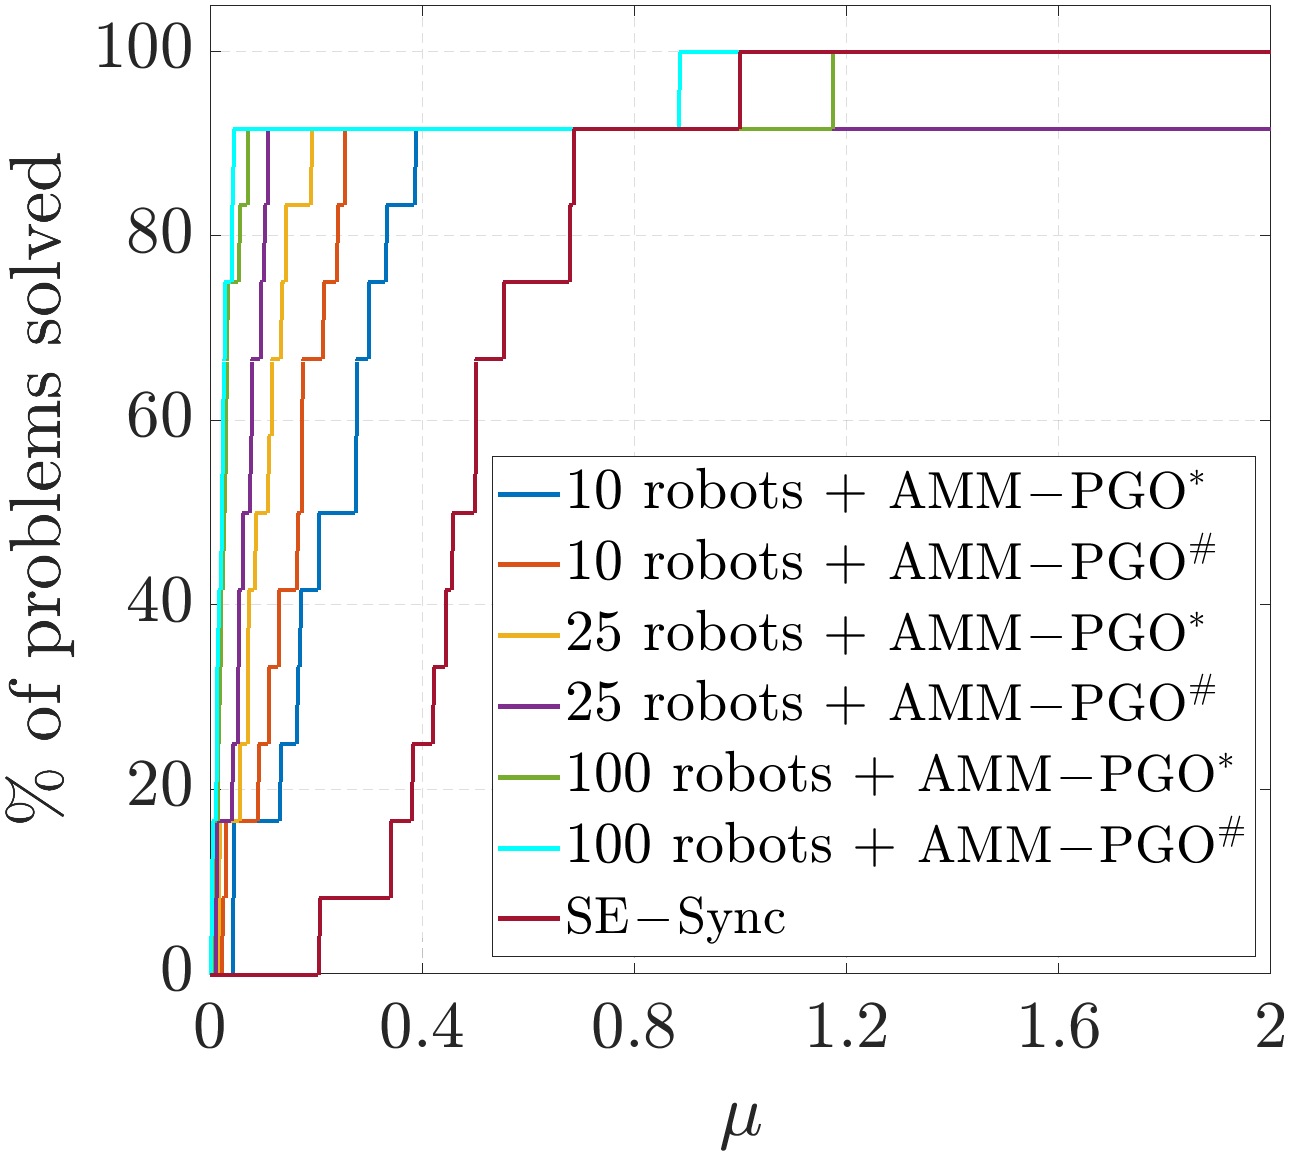
\includegraphics[trim =0mm 0mm 0mm 0mm,width=0.24\textwidth]{figures/succ/succ_time_1.png}} &
		\hspace{-0.55em}\subfloat[][$\Delta=1\times10^{-3}$]{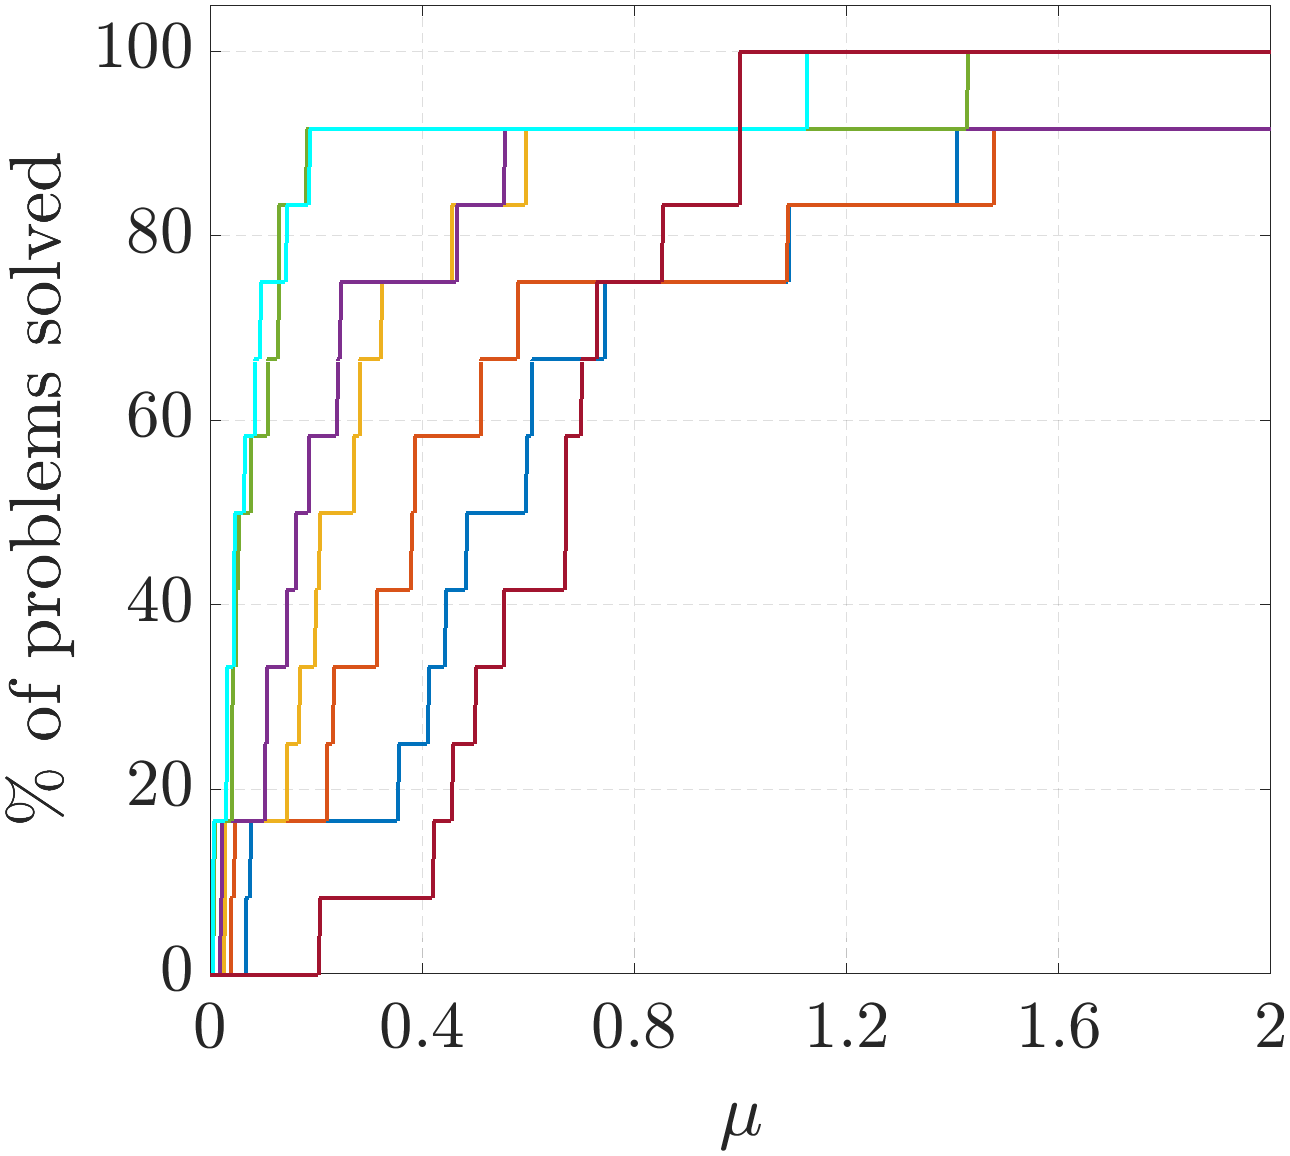
\includegraphics[trim =0mm 0mm 0mm 0mm,width=0.24\textwidth]{figures/succ/succ_time_2.png}} &
		\hspace{-0.55em}\subfloat[][$\Delta=1\times10^{-4}$]{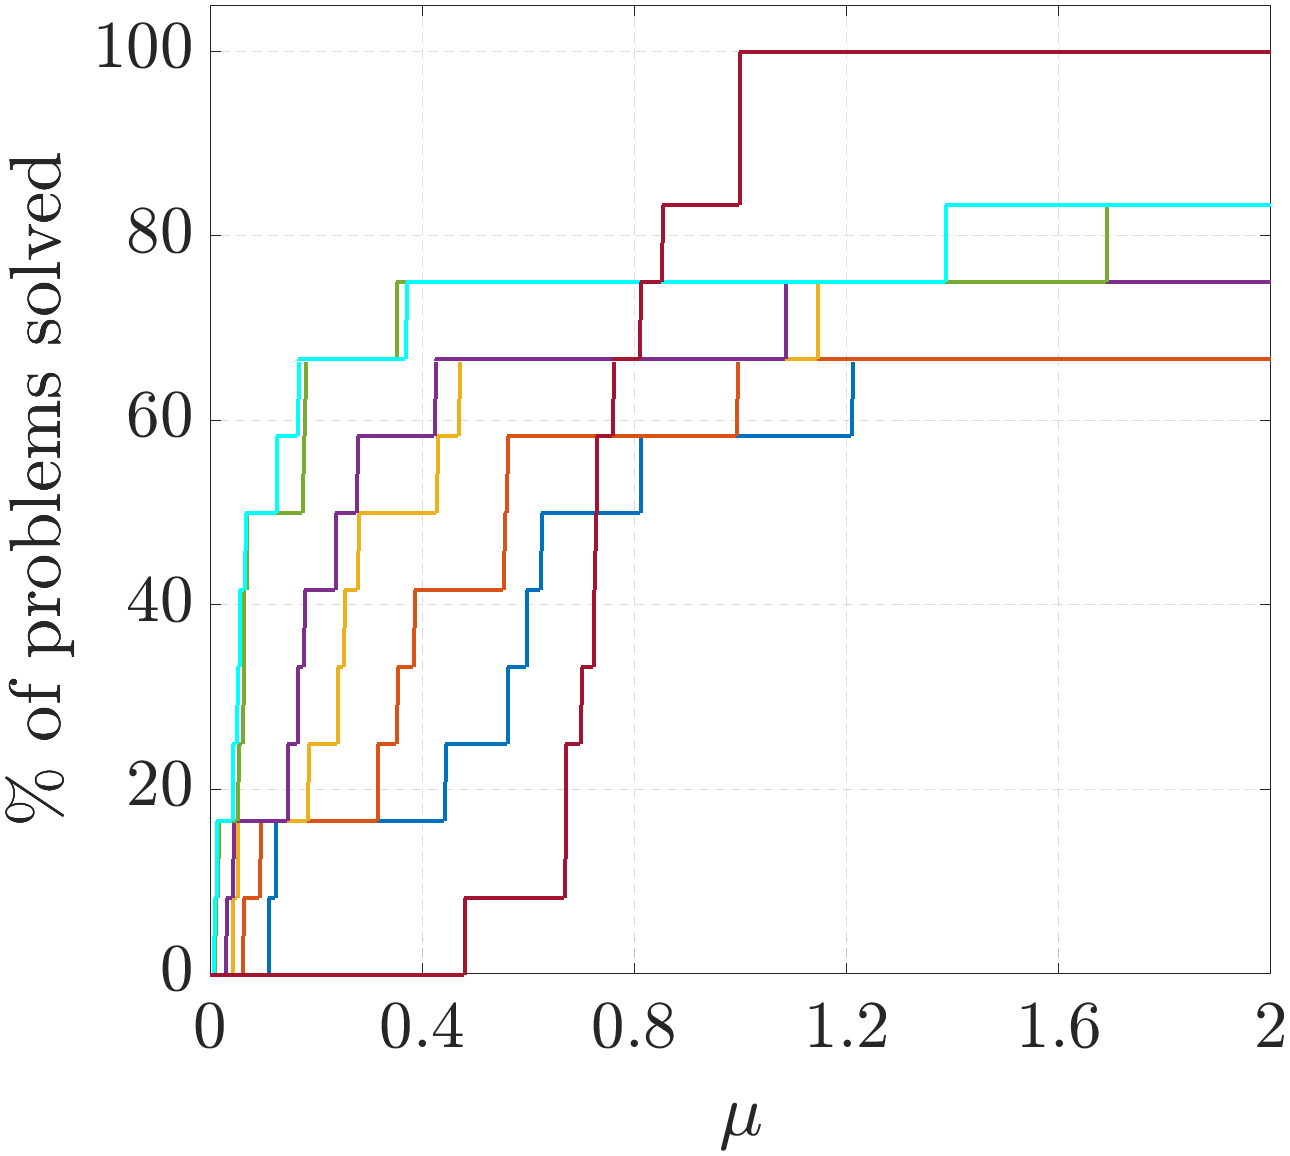
\includegraphics[trim =0mm 0mm 0mm 0mm,width=0.24\textwidth]{figures/succ/succ_time_3.png}}&
		\hspace{-0.55em}\subfloat[][$\Delta=1\times10^{-5}$]{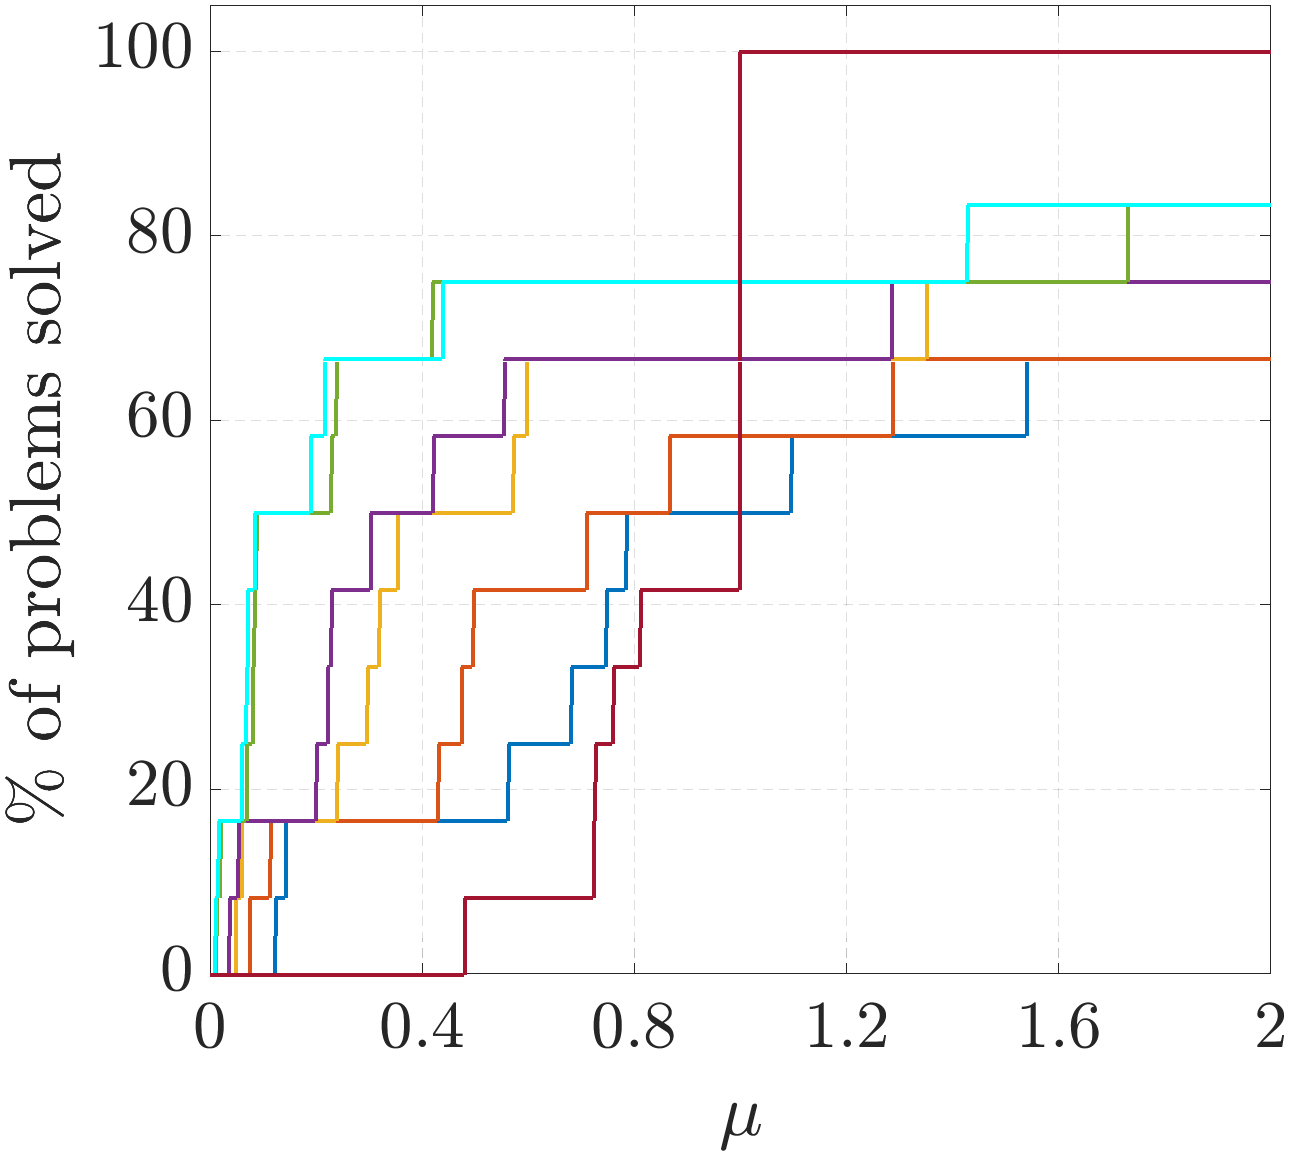
\includegraphics[trim =0mm 0mm 0mm 0mm,width=0.24\textwidth]{figures/succ/succ_time_4.png}}
	\end{tabular}
	\caption{Performance profiles for $\ammc$, $\ammd$ and $\sesync$ \cite{rosen2016se} on 2D and 3D SLAM benchmark datasets (see \datasetinfo). The performance is based on the scaled average optimization time per node $\ratio\in[0,\,+\infty)$ with  tolerances $\Delta=1\times10^{-2}$, $1\times10^{-3}$, $1\times10^{-4}$, $1\times10^{-5}$. The distributed PGO has 10, 25 and 100 robots (nodes) and is initialized with the centralized  chordal initialization \cite{carlone2015initialization}. Note that $\sesync$  solves all the PGO problems globally at $\ratio =1$. }\label{fig::succ_time}
	\vspace{-1.em}
\end{figure*}